%%%%%%%%%%%%%%%%%%%%%%%%%%%%%%%%%%%%%%%%%%%%%%%%%%%%%%%%%%%%%%%%%%%%%%%%
%    INSTITUTE OF PHYSICS PUBLISHING                                   %
%                                                                      %
%   `Preparing an article for publication in an Institute of Physics   %
%    Publishing journal using LaTeX'                                   %
%                                                                      %
%    LaTeX source code `ioplau2e.tex' used to generate `author         %
%    guidelines', the documentation explaining and demonstrating use   %
%    of the Institute of Physics Publishing LaTeX preprint files       %
%    `iopart.cls, iopart12.clo and iopart10.clo'.                      %
%                                                                      %
%    `ioplau2e.tex' itself uses LaTeX with `iopart.cls'                %
%                                                                      %
%%%%%%%%%%%%%%%%%%%%%%%%%%%%%%%%%%
%
%
% First we have a character check
%
% ! exclamation mark    " double quote  
% # hash                ` opening quote (grave)
% & ampersand           ' closing quote (acute)
% $ dollar              % percent       
% ( open parenthesis    ) close paren.  
% - hyphen              = equals sign
% | vertical bar        ~ tilde         
% @ at sign             _ underscore
% { open curly brace    } close curly   
% [ open square         ] close square bracket
% + plus sign           ; semi-colon    
% * asterisk            : colon
% < open angle bracket  > close angle   
% , comma               . full stop
% ? question mark       / forward slash 
% \ backslash           ^ circumflex
%
% ABCDEFGHIJKLMNOPQRSTUVWXYZ 
% abcdefghijklmnopqrstuvwxyz 
% 1234567890
%
%%%%%%%%%%%%%%%%%%%%%%%%%%%%%%%%%%%%%%%%%%%%%%%%%%%%%%%%%%%%%%%%%%%
%
%    J.-L. Ley
%
\documentclass[11pt]{iopart}
\newcommand{\gguide}{{\it Preparing graphics for IOP journals}}
%Uncomment next line if AMS fonts required
%\usepackage{iopams}  
\usepackage[english]{babel}
% \usepackage[latin1]{inputenc}
\usepackage[T1]{fontenc}	% accent dans le pdf
%\usepackage[utf8x]{inputenc}
\usepackage{colortbl}

\usepackage{caption}
\usepackage{tabularx} % Pour avoir des tableaux d'une largeur bien d�finie
\usepackage{graphicx} 
\usepackage{amsfonts}
 \usepackage{subfig} % Pour avoir des sous-figures.
\usepackage{multirow}
\usepackage{lscape}
\usepackage{pdflscape}
\usepackage{footnote}
%\usepackage{amsmath}

\usepackage{hyperref}

\hypersetup{
colorlinks=true, %colorise les liens
breaklinks=true, %permet le retour � la ligne dans les liens trop longs
urlcolor= blue, %couleur des hyperliens
% linkcolor= red, %couleur des liens internes
linkcolor= black, %couleur des liens internes
citecolor=blue, %couleur des r�f�rences
} 

% Package pour gerer les commentaires dans la marge
\usepackage{xargs} % Use more than one optional parameter in a new commands
\usepackage[colorinlistoftodos,prependcaption,textsize=scriptsize]{todonotes}
% \usepackage[disable,colorinlistoftodos,prependcaption,textsize=scriptsize]{todonotes}
\newcommandx{\com}[2][1=]{\todo[linecolor=blue,backgroundcolor=blue!25,bordercolor=blue,#1]{#2}}



\begin{document}

\title{Monitoring Ion Therapy with a Compton Camera: Simulation Studies of the Clinical Feasibility}

\author{J.-L.~Ley$^1$, D.~Dauvergne$^3$, N.~Freud$^2$, J.~Krimmer$^1$, J.~M.~L\'etang$^2$, V.~Maxim$^2$, M.-H.~Richard$^1$, and \'E.~Testa$^1$}

\address{$^1$Univ Lyon, Universit\'e Claude Bernard Lyon 1, CNRS/IN2P3, Institut de Physique Nucl\'eaire de Lyon, 69622 Villeurbanne, France}
\address{$^2$Univ Lyon, INSA-Lyon, Universit\'e Claude Bernard Lyon 1, UJM-Saint \'Etienne, CNRS, Inserm, Centre L\'eon B\'erard, CREATIS UMR 5220 U1206, F-69373, Lyon, France}
\address{$^3$LPSC, Universit\'e Grenoble-Alpes, CNRS/IN2P3 UMR5821, F-38026 Grenoble, France}
\ead{jeanluc.ley@gmail.com}

\begin{abstract}
The aim of irradiation monitoring during a treatment in ion therapy is to control in real time the agreement between the delivered dose and the planned treatment. In fact, the discrepancies might come from uncertainties such as the planning accuracy by itself, or by variations due to the positioning or the anatomical changes of the patient. This can lead to ion-range variations of a few millimeters.\com{This first part should be shorter (just speak about treatment uncertainties} Several devices are under development over the world to detect secondary radiation, which are correlated to the dose deposited by incident ions [1]. Compton cameras are in particular investigated for their potential high efficiency to detect prompt-gammas [2-5]. The present work aims at discussing the clinical applicability of a Compton camera design by means of Monte Carlo simulations validated against measurements of single and coincidence rates.\com{There is no validation of the simulation against experimental data. The abstract should provide a summary of the paper results}

\end{abstract}


%Uncomment for PACS numbers title message
%\pacs{00.00, 20.00, 42.10}
% Uncomment for Submitted to journal title message
\submitto{\PMB}
% Keywords required only for MST, PB, PMB, PM, JOA, JOB? 
\vspace{2pc}
\noindent{\it Keywords}: Compton Camera, ion therapy, clinical applicability, Prompt gamma
% Comment out if separate title page not required
\maketitle
%
\newpage

\tableofcontents

\newpage

\section{Introduction}\label{section::Intro}
Ion beam therapy is a cancer treatment technique which is rapidly gaining importance in the global tumor therapy panorama. In addition to the already operational 70 clinical facilities, for more than 175000 patients already treated by the end of 2017, several new centers have been designed and approved for construction worldwide~\cite{PTCOG_stats}. The favorable feature of this treatment technique is connected to the peculiar energy deposition profile of charged particles as a function of depth in matter. As first observed by Bragg~\cite{Bragg_main}, the depth-dose profile of charged particles shows a maximum close to the end of their range in matter; in addition to this, a strong enhancement of the relative biological effectiveness (RBE - capability of inducing DNA damages at fixed dose) is observed for ions heavier than protons in the region of the Bragg peak~\cite{RBE_Elsasser, RBE_Weyrather}, which enables a reduction of the biological dose in healthy tissues.

The Bragg peak position corresponds to the maximum of the dose deposited in the patient and must be tuned to cover the target volume and, at the same time, spare the surrounding healthy tissues. The tumor volume is defined via CT scan in the standard clinical routine, and the treatment is planned via treatment planning software. In human body, the exploitation of the high ballistic precision of ion beams is strongly limited by treatment planning and delivery uncertainties, like uncertainties in the material composition determination, CT units conversion to ion stopping power, patient mis-positioning, organ motion or morphological changes between treatment fractions (a standard treatment is divided into several fractions over several weeks, according to the tumor and patient characteristics). These uncertainties force the clinicians to fix relatively large safety margins around the planned treatment volume, up to 3.5\% + 3 mm~\cite{Paganetti:2012aa}. The research and clinics community agrees on the fact that ion-range verification is one of the conditions (at present the main condition) required for a broader usage of ion beam therapy and for its further development. With the goal of fully exploiting the ion beam therapy dosimetric potential, the monitoring should be in real-time and ideally in 3 dimensions, in order to be able to interrupt the treatment in case of severe issues, corresponding to important differences between the planned and delivered dose to the target volume or to surrounding organs, in particular in case of proximity to organs-at-risk~(OAR).

Several techniques have been considered worldwide for twenty years. Most of the studied techniques rely on the detection of secondary radiations generated during the slowing down process of incident ions, in particular during nuclear reactions. Among theses secondary radiations, positron emitters have been deeply studied in order to exploit positron emission tomography (PET) machines for treatment monitoring. PET techniques are based on the detection of the two back-to-back 511~keV photons produced by the annihilation of positrons (created by the emitter fragments of nuclear reactions) with patient electrons, resulting in a delayed radiation which should be detected with time coincidences, allowing for an intrinsic background reduction. Nevertheless, the monitoring with positron emitters secondary signal must deal with a limited count rate compared to medical imaging PET, with the lifetime of emitters providing a delayed information that implies the signal integration over a whole treatment fraction (not a single spot or group of spots), with physiological washout effects depending on to the emitters lifetime.

Even if the only available and functional range monitoring system in a clinical center is based on this technique~\cite{ENGHARDT2004}, several clinical experience with commercial or adapted PET system already shown intrinsic limitations mainly connected to the ring geometry (not directly applicable to the treatment monitoring due to the presence of the beam) or in general to geometrical constraints limiting the field of view and the resulting system global efficiency and spatial accuracy (the limited detection angle generates artifacts in the final image)~\cite{PARODI2016}. The research is ongoing and new results are expected for the next years thanks to the introductions of new systems with adapted geometries, to the improvements in acquisition and reconstruction techniques and to the clinical introduction of time-of-flight systems, intrinsically able to improve the detector spatial resolution via interaction time information, and depth-of-interaction reconstruction, which will allow for a more precise spatial reconstruction for reduced angular artifacts effects.

In addition to positron annihilation products, a different kind of photons is emitted during ion irradiation. They emerge from the relaxation of excited nuclei in a wide energy range, between some hundreds of keV till about 8-10 MeV. After the first idea proposal published in 2003~\cite{PG_first}, these secondary products of particle treatment have been deeply investigated and the correlation of this gamma radiation to the ion depth-dose profile has been confirmed by several research groups, starting from~\cite{Min_PG} for protons and~\cite{Testa_PG} for heavier ions (mainly carbon). The so-called prompt gamma-rays (PG) have the advantage to be emitted almost instantaneously after the beam interaction in the tissue, making them more adapted than PET 511~keV gammas for real-time monitoring. Consequently, different techniques have been proposed to exploit this signal for treatment monitoring purpose, with the related detection systems. Some methods are based on PG timing~\cite{Golnik:2014aa, Krimmer_PGPI} or energy~\cite{Verburg:2014aa} information and rely on non-collimated systems; more complex detection apparatus can achieve an actual PG imaging, by exploiting mechanical or electronic collimation (i.e.~with collimated gamma camera or Compton camera, respectively) for the photon selection (see e.g.~\cite{Min_PG, Bom_collimated, Smeets:2012aa, Roellinghoff_2014, Priegnitz:2015aa, Frandes_2010, LLOSA2012105, KORMOLL2011114, MCCLESKEY2015163, Matsuoka:2014qna, Peterson:2010aa, Solevi:2016aa, ALDAWOOD2017190}). For a review on PG monitoring, see~\cite{krimmer:hal-01585334}

Originally designed for astrophysics applications, the potential of Compton cameras for medical imaging has been soon recognized~\cite{TODD:1974aa} and then directly translated to the ion beam therapy monitoring domain. Such a gamma detection system is generally  composed of two sections: a scatterer and an absorber. The scatterer is dedicated to the gamma Compton scattering, and should be so adapted in order to optimize the Compton scattering probability in the prompt gamma energy range, while reducing the so called Doppler broadening effect due to electron bounding and motion~\cite{Doppler}; this leads, in most of the cases, to the choice of a light material (low $Z$), segmented in several subsections. However, when efficiency has to be privileged, heavier materials may be used~(\cite{Solevi:2016aa, ALDAWOOD2017190, 0031-9155-60-18-7085}). The absorber is devoted to the final absorption of the Compton scattered photons via photoelectric effect; it is often composed of segmented high-$Z$ scintillating materials. Slightly different Compton camera configuration can also achieve Compton electron tracking in the scattering detector~\cite{Frandes_2010, Yoshihara_ETCC}, which results in additional information for the further reconstruction algorithm.
 The collected interaction positions and energy depositions in the two detector sections are used to limit the emission point on the surface of a cone (or to a segment in the cone if the Compton electron track information is retrieved), via Compton kinematics reported in equation~\ref{Compton_equation} (for an electron initially at rest):
\begin{equation}
\cos\theta\,=\,1-\frac{m_{e}c^{2}E_{1}}{E_{2}(E_{1}+E_{2})},
\label{Compton_equation}
\end{equation} 
where \(m_{e}c^{2} = 511\)~keV, \(E_{1}\) and \(E_{2}\) are the energies, respectively, deposited in the scatterer and the absorber. 
Once the cones are calculated, analytic or iterative algorithms are used to create the image of the prompt gamma emission distribution, with intrinsic 3 dimensional capability~\cite{McKisson3D, Kuchment:2016uiw}. 


Several sources of uncertainty and signal background are connected to this detection method. Considering a gamma interacting twice in the detector, i.e.~once in the scatterer and once in the absorber, a complete photon energy absorption is needed since the initial photon energy (\(E_{1}\)) is not known a priori and the reported formula assumes valid the relation in equation~\ref{energy_equation}:
 \begin{equation}
E_{0} = E_{1}+E_{2}.
\label{energy_equation}
\end{equation} 
An underestimation of the total initial energy (caused by a photon non-complete absorption in the absorber section or by the Compton electron escape from the scatterer section), leads to an underestimation of the Compton angle, so to a Compton cone reconstruction incertitude. For a three-interaction operating mode (making use of double scattered photons), the initial photon energy can be calculated analytically so that a complete absorption is not mandatory. In addition to this, the Compton kinematics formula does not take into account the initial bounding configuration of the Compton scattering electron, which creates a blur in the Compton angle reconstruction, resulting in the already cited Doppler broadening effect~\cite{Doppler}. Furthermore, the time structure of the incoming particles plays an important role due to the detection principle, which is based on time coincidences between the two detector sections. The final image accuracy then suffers from false coincidences, generated by two prompt gammas interacting in the same time window or by the contamination of different kind of secondaries, mainly neutrons and protons. It is clear that excellent detector time resolution can limit the amount of random coincidences, as well as different background rejection methods can be applied to select real coincidences~\cite{Draeger:2017aa}. Energy selections can be applied to the collected coincidences~\cite{Polf:2009aa, Hilaire:2016aa}, or the homogeneous neutron background can be reduced via time-of-flight information~\cite{Testa:2010aa}.

A French collaboration of 4 research institutions (Institut de Physique Nucleaire and Centre de Recherche en Acquisition et Traitement de l'Image pour la Sant\'e in Lyon, Laboratoire de Physique Subatomique et Cosmologie in Grenoble, Centre de Physique des Particules in Marseille) is focused on the design and development of gamma detectors for online ion beam therapy monitoring. The project includes the development and clinical test of a Compton camera prototype based on semiconductor and scintillator detectors~\cite{krimmer:hal-01101334}; the feasibility of its clinical application is studied in this work with Monte Carlo simulations.
 
In a previous study by Ortega and colleagues~\cite{Ortega:2015aa} a detailed analysis of the noise sources for Compton imaging in proton therapy monitoring is presented, and the clinical application of this method for detecting range shifts is tested. The simulation study, performed with a simple Compton camera prototype composed by multiple LaBr$_3$ layers with a ideal mono-energetic proton beam impinging on a PMMA phantom, showed the relative expected rate of prompt gammas and neutrons, and the resulting rate of random coincidences ranging from 19 \% to more than 60 \% depending on the beam energy and the coincidence time window. This amount of fake events leads to complex reconstruction scenarios, where the identification of a 3~mm range shift is not clear for all cases.
    
Starting from these results, the ClaRyS camera performances are here studied as a function of the gamma energy in the prompt gamma energy range, and the possible application of this detector as depth-dose profile monitor during ion beam therapy clinical treatment is analyzed by investigating the effect of the beam time structure on the rate of true and random coincidences, as well as on the background level. After a preliminary study with point-like gamma sources irradiation focused on detector efficiency measurements as a function of the source position and gamma energy, clinical proton and carbon beams impinging on an homogeneous PMMA phantom are simulated to reproduce treatment conditions and analyze the prompt gamma detection resulting scenario. A beam intensity reduction with respect to treatment intensities is studied for monitoring purpose, with the aim of increasing the ratio between true and random coincidence events: the maximum beam rate tolerance is here estimated. Two kinds of reconstruction algorithms, a line-cone analytic method and a MLEM iterative one, are applied to the collected data in order to compare the imaging results. Finally, the Compton camera precision in the identification of the dose profile fall-off is reported.   



\section{Material and methods}

\subsection{Simulation setup}

The monitoring system modeled in this simulation work is a Compton camera prototype under development within the French collaboration CLaRyS. The detectors detailed characteristics can be found in \cite{krimmer:hal-01101334}. A scheme of the simulation setup is given in figure~\ref{fig:fig_setup_CC_simulation_Hadronth}.

\begin{figure}	
  \centering
  \includegraphics[width=0.7\textwidth]{./Figure/Compton_Camera_hadontherapy_PMMA_Cylinder_EN.pdf}
  \caption{Scheme of the simulation setup: a PMMA cylindrical phantom is set in front of the Compton camera prototype. The Compton camera is composed of a stack of 7 double sided silicon strip detectors (scatterer) and a plan of 100 single BGO blocks. The set distances are realistic for clinical conditions. This geometrical configuration has been used for all the simulations presented in this work.}
  \label{fig:fig_setup_CC_simulation_Hadronth}
\end{figure}

Like most of the Compton camera devices, the CLaRyS prototype includes a scatterer and an absorber. The scatterer consists of seven parallel planes of silicon detectors (double-sided silicon strip detectors, DSSDs), $9\times9\times0.2$~cm$^3$, with 1~cm distance between the centers of two neighboring planes, while the absorber is composed of an array of $10\times10$ BGO (Bismuth Germanate - Bi$_{12}$GeO$_{20}$) blocks ($3.5\times3.5\times3.0$~cm$^3$ each) placed behind the silicon layers at a distance which can be tuned according to the requirements.\\ 
The silicon detectors have a strip pitch of 1.4~mm, for a total of 64 strips per side (double-sided readout based on electron and hole pairs collection). 
Regarding the BGO blocks, their entrance surface is streaked in a 8$\times$8 matrix of pseudo-pixels, 4.4$\times$4.4~mm$^{2}$ size, and the readout is performed via 4 photo-multiplier tubes. The position reconstruction is achieved via Anger logic.\\

In the simulation setup, the ion beam interacts with a cylindrical PMMA (PolyMethylMethAcrylate) phantom (15~cm diameter and 20~cm length) placed in front of the Compton camera as target. It is placed 20~cm far from the first silicon plane (center-to-center distance) in order to exit to a patient in the treatment room. The distance between the last silicon layer and the absorber array (center-to-center) is set to 40~cm.\\
The silicon detector strips are not reproduced in the simulation code, and the transverse spatial resolution is set to 0.9~mm FWHM at the reference energy of 1~MeV, according to preliminary measurements performed on smaller detector prototypes. Concerning the transverse direction (perpendicular to the beam line), the interaction position is set to the center of the involved silicon plane. A mono-block crystal is simulated for the absorber for simplicity. The events are selected to be limited to a single block component based on the interaction localization, and the interaction position is reconstructed via center of gravity calculation if multiple interaction occur. An incertitude contribution, randomly extracted by a Gaussian of 5~mm FWHM , is added to the reconstructed position to fit with the geometrical features. For what concerns the parallel direction, given the fact that the employed BGO blocks have not depth of interaction reconstruction capabilities, the interaction position is fixed to the center of the mono-block crystal.\\
The energy resolution of the BGO blocks was estimated in preliminary measurements and is accordingly set to 17\% FWHM at the reference energy of 667~keV (a 137-cesium source has been used for the measurements). The energy resolution of the silicon detector is set to 2.3~keV (RMS) according to the design expectations; no characterization data are yet available for an instrumental estimate.

The time resolution has been set to 3.0~ns FWHM for the BGO blocks and to 15.0~ns FWHM for the silicon slabs, according to preliminary measurements performed on test detector modules at the GANIL %(Grand Accelerateur National d'Ions Lourds) 
center in France.

The detector resolutions play an important role in the Compton camera performances. The spatial resolution of the absorber influences the position of the apex of the Compton cone as well as its axis orientation. The energy resolution of the scatterer determines the Compton cone aperture angle. The time resolution impacts the coincidence window between the absorber and the scatterer, and therefore the detectors ability to distinguish between true and random coincidences.

The CLaRyS project also includes the development of a beam tagging hodoscope, composed of scintillating fibers read out by multi-channel photomultipliers. This detector is used to synchronize the beam time and space structure to the prompt gamma detection in order to tune the detection window reducing the background contamination. The hodoscope is not included in the simulation, but its time resolution has to be taken into account for the time-of-flight discrimination (see section~\ref{MatMeth::TOF_Ecut}). It is set to 1~ns FWHM. \\
The detector's spatial, energy, and time resolutions are summarized in table \ref{table:table_resolution_detecteurs_CC_simulation_Hadronth}.

\begin{table}
\centering
%\begin{tabular}{>{\columncolor[gray]{0.9}}ccc}
\caption{Estimations of reachable resolutions with the detectors. Those resolutions are applied during the simulations.}
\begin{tabular}{cccc}
\hline
\textbf{Resolution (FWHM) at 1 MeV} & \textbf{Scatterer} & \textbf{Absorber} & \textbf{Hodoscope}\\
\hline 
\textbf{spatial [mm]	}			 &     0.9		 &  5 &	 1\\
%\hline
\textbf{energy}				&	2.3~keV		&  17~\%	&	/\\
%\hline
\textbf{timing [ns]}	        		&	15			&	3 	&  1\\
\hline
\end{tabular}
\label{table:table_resolution_detecteurs_CC_simulation_Hadronth}
\end{table}
    
The Monte Carlo simulation is performed with the Geant4 toolkit, version 9.6 patch 02. 
%Geant4 has been developed at CERN %(Conseil europ\'{e}en pour la recherche nucl\'{e}aire) for high energy physics experiments, but it has been shown that it can be used for ion beam therapy studies \cite{cirrone_hadrontherapy_2011,toshito_new_2010}. 
%Some improvements are still needed in order to extend the hadronic models to low energy applications~\cite{dedes_assessment_2014, Pinto:2016aa}.

The particle interactions in matter are described in this work by means of the models listed in table~\ref{table:table_modele_physic_CC_simulation_Hadronth}. Additionally, the Doppler broadening and the photon polarization effects are taken into account.
 

\definecolor{Gray}{gray}{0.9}

\begin{table}
\label{physlist_ion}
\caption{Hadronic models used in the Geant4 simulations.}
\begin{scriptsize}
\begin{center}
\renewcommand{\arraystretch}{1.2}
%\begin{tabular} {>{\columncolor[gray]{0.9}}cccc}\hline  
\begin{tabular} {cccc}\hline
%\rowcolor{Gray}
\textbf{Process} & \textbf{Protons} & \textbf{Ions} & \textbf{Neutrons} \\ \hline 
\textbf{Electromagnetic} & \multicolumn{3}{c}{standard$_{\rm{option3}}$} \\ %\hline
\textbf{Inelastic} & G4BinaryCascade & G4QMDReaction  &  G4BinaryCascade  \\ 
 & & (G4IonsShenCrossSection)&+ G4NeutronHPInelastic ($<$19 MeV)\\ %\hline
\textbf{Elastic} & G4LElastic & G4LElastic & G4LElastic + G4NeutronHPElastic ($<$19 MeV)\\ %\hline
\textbf{Fission} & / & / & G4LFission + G4NeutronHPFission($<$19 MeV) \\ %\hline
\textbf{Capture} & / & / & G4LCapture +  G4NeutronHPCapture ($<$19 MeV) \\ %\hline
\textbf{Radioactivedecay} & / & G4Radioactivedecay & / \\ \hline
\end{tabular}
\end{center}
\end{scriptsize}
\label{table:table_modele_physic_CC_simulation_Hadronth}
\end{table}

The two main beam particles used in clinics are considered: protons and carbon ions. The beam range of interest is 15.2~cm in the PMMA phantom, and the associated energy is 160~MeV for protons and 305~MeV/n for carbon ions.
 
The beam transverse dimension is modeled with a Gaussian distribution with a standard deviation of 5~mm for protons at 160~MeV and 3.5~mm for carbon ions at 305~MeV/n. The beam intensity for a spot in pencil beam scanning (PBS) mode is $10^8$ for protons and $10^5$ for carbon ions. The beam time structure is applied at the data analysis stage and described in section~\ref{subsubsection:modelisation_fasceau_ions_CC_hadrontherapy_Geant4}.\newline

%\subsection{Data processing}
%\label{subsection:Treatment_data_CC_hadrontherapy_Geant4}

\subsection{Beam time structure}
\label{subsection:modelisation_fasceau_ions_CC_hadrontherapy_Geant4}
 
Two different beam time structures have been considered for this study, related to two kinds of accelerators used in clinical practice: the IBA C230 cyclotron for protons (used in 16 clinical centers worldwide) and the synchrotron installed in the Heidelberg Ion Therapy Center (HIT), Germany, for carbon ions. For protons at 160 MeV, the primary particles are grouped in bunches of 2~ns (this value may vary also according to the distance between the cyclotron and the treatment room, and energy spread selection) at a frequency of 106~MHz (9.42~ns)~\cite{f_roellinghoff_real-time_2014}. The clinical beam intensity is 3.2~nA which corresponds to about 200 protons per bunch. Concerning the carbon ion beam at 305~MeV/u, the estimated microstructure is composed of 30~ns duration bunches at a frequency of 5.9~MHz (170~ns period). The clinical beam intensity for carbon ions is $5\times10^7$~ions/s, corresponding to about 9~ions per bunch. This beam structure is extrapolated from measurements performed by our group in 2013 at HIT; the beam time structure was measured for 200~MeV/u and 400~MeV/u primary ion energy with a two-fiber hodoscope (basic prototype of the one at present under development) and the spill signal was given by the accelerator. Figure \ref{fig:fig_structure_temps_faisceau_HIT_2013_CC_simulation_Hadronth} shows the beam structure for carbon ions at 400~MeV/u. The pulses have a spill period of 150.2~ns and each bunch is approximately 21.5~ns.
The mentioned measurements have shown that the spill phase changes during the extraction: this implies that the HF signal from the synchrotron can not be used to trigger the pulses, so that the use of an additional beam time stamp system like the hodoscope seems required for time-of-flight background rejection purposes.\newline

	\begin{figure} [!hbtp]	
	\centering
	\includegraphics[width=0.5\textwidth]{./Figure/2013_Structure_Time_Beam_400MeV.png}
	\caption{Time micro-structure measured from a carbon ion beam at 400~MeV/u delivered at HIT. The pulses have an extraction period of 150.2~ns and the bunches are 21.5~ns FWHM. The measurement was achieved with a two-scintillating-fiber hodoscope.}
	\label{fig:fig_structure_temps_faisceau_HIT_2013_CC_simulation_Hadronth}
	\end{figure}


The coincidence window (between scatterer and absorber events) is set to 40~ns, centered on each absorber detected interaction. This value is adapted to the detectors time resolutions. Table~\ref{table:definition_beam_structure_CC_hadrontherapy_Geant4} summarizes the presented beam time structures and coincidence reconstruction features.

\begin{table} [!htbp]
\footnotesize
\centering
\caption{Description of the two beam structures studied: the IBA cyclotron C230 for protons and the synchrotron installed at the Heidelberg Ion Therapy Center (HIT) in Germany for carbon ions. The macro-structure of the synchrotron, at the second time scale, is not considered here. The beam structures are applied to the simulation data.}
\setlength{\tabcolsep}{2pt}
%\hspace{-2.1cm}
\begin{tabular}{c|c|cc}
%\cline{2-4}
\hline
		\multicolumn{2}{c}{ }		 & 					\textbf{Protons} & \textbf{Carbon ions}\\ 
\hline
%\cline{2-4}%\hline
\multirow{3}{*}\textbf{Clinical features}		&	Facility	& IBA Cyclotron C230 &   Synchrotron at HIT\\
											& Clinical intensity& $  2\times10^{10}$ p/s  & $  5\times10^{7}$ ions/s\\
											& Energy 			&160 MeV 			&    305 MeV/u\\
%\cline{2-4}%
\hline
\multirow{3}{*}\textbf{Beam structure}		&	Bunch time [ns]	& 3.2				&  30\\
											& Period [ns]		&   9.4 				& 170\\
											& Primaries /bunch 	&217 			& 9\\
%\cline{2-4}%
\hline
\multirow{2}{*}\textbf{Detectors}						& Coincidence window [ns]		& 40 	&  40 \\
											&Time resolution [ns] & \multicolumn{2}{c}{Si: 15 and BGO: 3}\\
%\cline{2-4}%
\hline
\end{tabular}
\label{table:definition_beam_structure_CC_hadrontherapy_Geant4}
\end{table}



\newpage
%---------------------------------------------------------------
%---------------------------------------------------------------
\subsection{TOF and energy based data selection}
\label{MatMeth::TOF_Ecut}

The Compton detection principle is based on a double interaction in the scatterer and absorber section, where an interaction is defined as an energy deposit in a detector module. As discussed in section~\ref{subsubsection:modelisation_fasceau_ions_CC_hadrontherapy_Geant4}, the coincidence reconstruction relies on a defined time window, fixed according to the detector resolution. In a simulation environment, different kinds of coincidences events can be distinguished and studied: 
\begin{itemize}
\item[-] real coincidences: created by a single photon first interacting in a single scatterer plane and then in a single absorber block;
\item[-] quasi-simultaneous interaction of two secondary particles;
\item[-] double interaction of the same particle, not a photon (protons, neutrons).
\end{itemize}

In an experiment the collected data are affected by a certain number of the so-called random coincidences, which cannot be experimentally distinguished form true coincidences. The amount of random coincidences depends on the detector time resolutions, on the fixed time coincidence window and on the beam time structure, on the phantom composition and camera prototype setup. In figure~\ref{fig:fig_explication_coincidence_CC_simulation_Hadronth}, a schematic view of the different kinds of coincidences is presented.

\begin{figure}
  \centering
  \includegraphics[width=0.9\textwidth]{./Figure/Schema_coincidence_EN.eps}
  \caption{Diagram showing the different definitions of coincidences in the Compton camera.}
  \label{fig:fig_explication_coincidence_CC_simulation_Hadronth}
\end{figure}

In addition to this, the prompt gamma measurement is contaminated by other secondary particles (mainly massive and charged particles like protons and neutrons), produced by the interaction of the primary particles with the patient/phantom.\\
Ad-hoc filtering methods are applied to reduce the above described contamination.

\begin{itemize}
\item Time-Of-Flight: it has been demonstrated by our group that a time-of-flight discrimination is possible and effective in reducing the background generated by massive particles interactions~\cite{Testa:2010aa}. The photons are moving at approximately the speed of light while the massive particles approach the detector at a lower speed. The time information provided by the hodoscope and the absorber can be combined to fix a detection time window and reject all the events outside the window. The time between the incident particle creation and the secondary particle detection in the absorber is considered as the time-of-flight. The hodoscope time resolution $u_{\mathrm{hodoscope}}$ (1~ns FWHM) is applied to the primary particle creation time, with a contribution randomly extracted from a Gaussian with $\sigma\,=$ 1/2.35~ns. The detection time in the absorber is affected by the absorber time resolution.

 \begin{eqnarray}
TOF_{\mathrm{theoretica}} = t_{\mathrm{absorber}}-t_{\mathrm{hodoscope}} \\
TOF_{\mathrm{simulation}} = t_{\mathrm{absorber}}+t_{\mathrm{creation}} + u_{\mathrm{hodoscope}}
\label{TOF_equation}
\end{eqnarray} 

The time-of-flight spectrum resulting from the simulation shows that the coincidences of interest (produced by prompt-gamma rays) are included in a window between 0 and 8~ns (figure \ref{fig:fig_TOF_distribution_CC_simulation_Hadronth}). Therefore, all the coincidences with a TOF higher than 8~ns have been rejected.
\begin{figure}	
  \centering
  \includegraphics[width=0.6\textwidth]{./Figure/2015_01_04_TOF_spectra_NoCut_1Proton_ResolTemporelle_applied_these.jpg}
  \caption{Time of flight spectrum obtained by means of the simulation for a proton beam at 160 MeV and $1\times10^{8}$ incident protons. The detection time for the absorber is given by the tag for the first deposit energy. The blue curve represents the time of flight for true events and the black one represents the background.}	
  \label{fig:fig_TOF_distribution_CC_simulation_Hadronth}
\end{figure}

\item Energy selection: energy thresholds are defined for the event detection. 50~keV and 100~keV are set as lower threshold for the energy deposited in a single silicon layer and absorber, respectively. For a complete event, a total absorbed energy lower limit is set to 1~MeV. In addition to the effect of background rejection, this selection also reduces the impact of partially absorbed photons and events with Compton electron escape.

\end{itemize}

\subsection{Reconstruction algorithms}
\label{MatMeth:reconstruction}
Once the coincidences are defined and selected according to the fixed physical cuts, the prompt-gamma emission point has to be reconstructed for each event. This can be done via analytic or iterative algorithms based on the Compton kinematics. Both are presented in the following sections.


\subsubsection{Line-cone algorithm}
The reconstruction via line-cone algorithm exploits the energy deposit and position information collected by the camera in addition to the beam planned path. Thanks to the deposited energies in the detectors and the interaction positions, a cone surface is analytically defined via the Compton equation~\ref{Compton_equation}. Figure~\ref{fig:reconstruction_scheme} shows a sketch of the reconstruction principle. The interaction position in the scatter gives the cone apex and the line connecting the interaction position in scatterer and absorber gives the cone axis. We assume that the initial energy of the gamma ray is fully absorbed in the absorber. In order to constrain the reconstruction, the beam direction is used to limit the possible solutions (lying on the reconstructed cone surface) to two points (intersection of the beam direction and the reconstructed cone). The set of all the reconstructed points gives the emission source distribution. The final image is the mono-dimensional projection of the prompt gamma emission spectrum. 

\begin{figure}
\centering
  \includegraphics[width=0.6\textwidth]{./Figure/reconstruction_scheme}
  \caption{Scheme of the reconstruction principle for Compton events. For line-cone reconstruction methods, two points are extracted for each event (diamonds in the figure), provided by the intersection between the reconstructed Compton cone and the beam line. The reconstructed image is strictly mono-dimensionale. For the iterative MLEM algorithm, each algorithm iteration adds constraints to the reconstructed cone surfaces, leading to  a three dimensional image.}	
  \label{fig:reconstruction_scheme}
\end{figure}

\subsubsection{LM-MLEM algorithm}	
The iterative methods allow to get a 3D image reconstruction, potentially by taking into account the spatial resolution and the energy resolution of the detectors. Few iterative algorithms have been developed for Compton event reconstruction~\cite{schone_common_2010, zoglauer_design_2011,gillam_compton_2011,mackin_evaluation_2012,lojacono_low_2013}.

The \textit{List-Mode Maximum Likelihood Expectation Maximization} (LM-MLEM) algorithm is an MLEM version which allows to reconstruct the image directly from the list of detected events.
The LM-MLEM algorithm used for this study is the one developed by the CREATIS research group in Lyon~\cite{maxim_filtered_2014,hilaire_compton_2014}.\newline%\cite{maxim_analytical_2009,lojacono_low_2013,maxim_filtered_2014,hilaire_compton_2014}.\newline
The first step is to define the volume which includes the origin of the prompt gamma ray detected. This volume is divided into equal voxels and the emission intensity is assumed homogeneous for each voxel $j$, with a Poisson distribution of parameter $\lambda_j$ (a vector of the emissions intensities of all the voxels). The algorithm is based on a system matrix $T$ composed of the coefficients  $t_{ij}$ which represent the probability that a photon produced in the voxel $j$ is detected in coincidence by the Compton camera as an event $i$. The probability for a gamma detected in coincidence to be emitted from the voxel $j$ is denoted as $s_j$.
The LM-MLEM algorithm starts with an initial value $\lambda^{(0)}_j$, which can be the simple back-projection reconstruction.
The iterations rely on the following recurrence relation:

\begin{equation}
\lambda_j^{(l+1)} =  \frac{\lambda_j^{(l)} }{s_j} \sum\limits_{i=1}^{N_{\gamma}} t_{ij} \frac{1}{P_i^{(l)}},\quad \rm{with}\quad  P_i^{(l)}=\sum\limits_{k=1}^{N_{v}} t_{ij}\lambda_k^{(l)},
 \label{eq:equation_lambda_compton_med_nucleaire}\newline
\end{equation}
where $N_{\gamma}$ is the number of detected events and $N_v$ is the number of voxels in the image.\newline

For each photon detected, the coefficients in column i are calculated by taking into account the uncertainties on the angle between the source and the involved scatterer plane and the angle between the scatterer plane and the absorber involved module.
The matrix elements $t_{ij}$ are calculated as:
\begin{equation}
 t_{ij} = K(\beta_i,E_{tot})\frac{|\rm{cos}(\theta_{{V_2V_1}}) |}{V_2V_1^2} \int\limits_{M\in v_j} \frac{|\rm{cos}(\theta_{V_1M})|}{V_1M^2} h_i(M)dv,
 \label{eq:equation_tij_compton_med_nucleaire}\newline
\end{equation}
where $\beta_i$ is the Compton scattering angle, $V_1$ the interaction position in the scatterer, $V_2$ the interaction position in the absorber, $h_i$ the spatial kernel which models the uncertainties on the Compton angle for each voxel $M$, $K(\beta_i,E_{tot})$ the differential cross section and $v_j$ the reconstructed volume.\newline

In order to simplify and speed up the calculation of the $t_{ij}$ matrix, the voxels located far from the reconstructed cone are set to 0. The distance between the cone and the voxel is calculated by taking the voxel center as reference point. \newline%The spatial resolutions are not included in this version of the algorithm.\newline
For each iteration, the matrix $T$ is stored and the reconstructed image can be produced.


\subsection{Performance study}
\label{MatMeth:performance}
In this section the parameters studied for the camera performance evaluation are explained. The study is mainly divided into three sections:
\begin{itemize}

\item Absolute efficiency: the camera absolute efficiency for gamma detection is studied by means of mono-energetic irradiation with point-like sources;
\item Rate of random coincidences: with proton and carbon beams interacting with the PMMA phantom, the rate of random and true detected coincidences is studied as a function of the beam intensity;
\item Camera precision: the camera capability of identifying the fall-off of the prompt-gamma emission profile is tested and the two reconstruction methods presented above are compared. 

\end{itemize}


\subsubsection{Absolute detection efficiency}
The absolute efficiency is crucial for the Compton camera performances and for its possible application in treatment monitoring. An efficient monitoring system should be ideally in real time, in order to allow for a treatment adaptation or interruption in case of severe issues detected in the delivered dose profile with respect to the planned treatment. In order to achieve an online detection of such deviations, given the reduced prompt gamma emission rate per incident ion~\cite{Ortega:2015aa}, an high detection efficiency is required to perform a monitoring on, ideally, a beam spot basis. In addition to this, the absolute detection efficiency directly affects the image reconstruction quality, which is in general increased for increased statistics.\\

In order to well define the expected camera efficiency, it has been studied with the irradiation from point-like monoenergetic gamma sources, set in different positions with respect to the center of the camera on the transverse plane.	

The absolute efficiency $\epsilon$ is defined as:
\begin{equation}
\epsilon =\frac{\mathrm{N}\gamma_{\mathrm{recons}}}{\mathrm{N}\gamma_{\mathrm{total}}},
\end{equation}
\label{eq:equation_efficacite_absolue}
with $N\gamma_{recons}$ the number of gamma events in coincidences, $N\gamma_{total}$ the total number of gamma emitted: $10^8$.\newline

The setup is the same as figure \ref{fig:fig_setup_CC_simulation_Hadronth}, with the exception of the PMMA phantom which is removed to leave the gamma source in air.
The point-like source is set in the range $-300$~mm to $+300$~mm (with the center of the camera transverse section set in the position 0) with a step of 20~mm close to the center of the camera, then increasing up to 1~cm for the most peripheral point. The movement followed the transverse axis of the camera. Different energies has been tested to mimic different prompt gamma spectroscopic lines: 300~keV, 500~keV, 1~MeV, 2~MeV, 4~MeV, 6~MeV. No time structure is reproduced for this part for the study.\newline

\subsubsection{Rate of random coincidences}

As the Compton detection principle relies on time coincidences, in addition to the main importance played by the detectors energy resolutions, the beam intensity and time structure are important parameters to be studied in order to asses the possible clinical implementation of a Compton detection based monitoring of ion beam treatment. The ability of the detection system to distinguish between true and random coincidences, i.e the resulting signal over noise ratio, strongly depends on the primary particle time structure. The number of true and random coincidences (where the two cases listed in section~\ref{MatMeth::TOF_Ecut} are included in the random coincidences) is studied as a function of the beam intensity, before and after data reconstruction via line-cone algorithm~(see section~\ref{MatMeth:reconstruction}).\\
In the simulation, the beam intensity is modeled by an average number of particles per bunch. The exact number of particles in each bunch is given by a random extraction from a Poisson distribution, where the mean value is the selected beam intensity. The range of intensities is defined in order to cover a wide range of operation: from a very low beam intensity to a realistic clinical particle rate. Therefore, for proton and carbon ions, the lowest beam intensity is set to 0.1 particles per bunch on average, while the upper limit is set to 217 protons or 70 carbon ions per bunch. All the simulations are performed with a total of $10^{8}$ primary protons and  $2\times10^{5}$ primary carbon ions. Those value correspond to realistic clinical values used for the treatment of a single spot (REFERENCE HERE - I DIDN'T FIND ANYTHING USEFUL). For the analysis of the results, the coincidence yields are scaled to the number of incident ions and the beam intensity to the average number of ions per bunch.

\subsubsection{Camera precision}
\label{MatMeth:precision}

The camera precision is defined as the difference between the predicted Bragg peak position (according to the treatment planning) and the detected Bragg peak position.\\
 
In this study, a reference profile has been defined as the reconstructed emission vertex profile at high statistics. This Bragg peak position is used as reference and compared to the ones reconstructed at lower statistics.

The high statistic profile has been obtained with $\mathrm{10^{10}}$ incident protons and reconstructed via line-cone algorithm~(figure~\ref{fig:fig_Results_Estimation_Camera_Profil_highStat_CC_simulation_Hadronth_LineCone}) and with the LM-MLEM reconstruction method~(figure~\ref{fig:fig_Results_Estimation_Camera_Profil_highStat_CC_simulation_Hadronth_MLEM}). To be noticed that the two reconstruction methods produce different results: the line-cone method is based on the beam direction information, so that it naturally produces a mono-dimensional image as result, while the MLEM method is able to reconstruct the prompt-gamma emission distribution in three dimensions. A projection along the beam direction is extracted from the MLEM reconstructed image in order to allow a direct comparison.\\  
The \textit{SmoothKern} method, with the Nadaraya-Watson regression~\cite{Nadaraya_regression, Watson_regression}, is used to smooth the reference profiles in order to reduce relative statistic fluctuations.\newline
A region of interest (ROI) ranging from $y=0$ mm to $y=+100$ mm is defined around the expected Bragg peak position, located at $y=+50$~mm in the phantom. The reference reconstructed profiles are modeled in the ROI by a linear combination of Non-Uniform Rational Basis Splines (NURBS)~\cite{NURBS}. \newline
Starting from the reference data set, data subsets at lower statistics are randomly extracted to mimic the dose profile falloff reconstruction for different primary particle statistics, in the range 1$\times$10$^8$ to 5$\times$10$^9$. The data subsets are directly extracted following a Poisson law from the reconstructed and smoothed reference profile, so that no further reconstruction is required.\\
For each chosen statistics, 1000 data subsets are extracted and the Migrad minimization method is applied to deduce the minimal shift between the reference profile and the one obtained from the data subset. The minimization algorithm shifts the reference profile in a 60~mm range, between $-30$~mm and $+30$~mm with respect to the initial position, with a step of $0.1$~mm, and for each position it compares its position to the low statistics profile by calculating the $\chi^2$ as follows:

\begin{eqnarray}
\chi^2 = \sum\limits_{i=1} {(y_{\mathrm{sample,i}}-y_{\mathrm{NURBS,i}})^2},
\end{eqnarray}

where $y_{\mathrm{sample}}$ is the number of coincidences for the low statistics profile, $y_{\mathrm{NURBS}}$ is the number of coincidences for the reference profile NURBS (scaled at the same low statistic) and i the step number.\newline
Figures~\ref{fig:fig_Results_Chi2_Distribution_Variation_CC_simulation_Hadronth_LC} and~\ref{fig:fig_Results_Chi2_Distribution_Variation_CC_simulation_Hadronth_MLEM} show the distribution of $\chi^2$ calculated for a low statistic profile at $10^8$ incident protons.\newline
The global minimum of all the calculated $\chi^2$ is then retrieved and the shift associated to this value is used to create the shift distributions shown in figure~\ref{fig:fig_Results_Precision_Distribution_Variation_CC_simulation_Hadronth_LC} and~\ref{fig:fig_Results_Precision_Distribution_Variation_CC_simulation_Hadronth_MLEM} for the line-cone and LM-MLEM algorithm respectively, for $10^8$ incident protons. The standard deviation of the distribution resulting of the thousand results gives the precision of the camera for a given number of incident protons. 


\begin{figure}
\centering
\subfloat[\label{fig:fig_Results_Estimation_Camera_Profil_highStat_CC_simulation_Hadronth_LineCone}]{\includegraphics[width=0.33\textwidth]{./Figure/profile_high_stat_linecone.pdf}}
\subfloat[\label{fig:fig_Results_Estimation_Camera_Profil_highStat_CC_simulation_Hadronth_MLEM}]{\includegraphics[width=0.32\textwidth]{./Figure/profileY_corr_r15.png}}\\
 %\subfloat[\label{fig:fig_Estimation_Camera_CC_NURBS_Poisson_LC}]{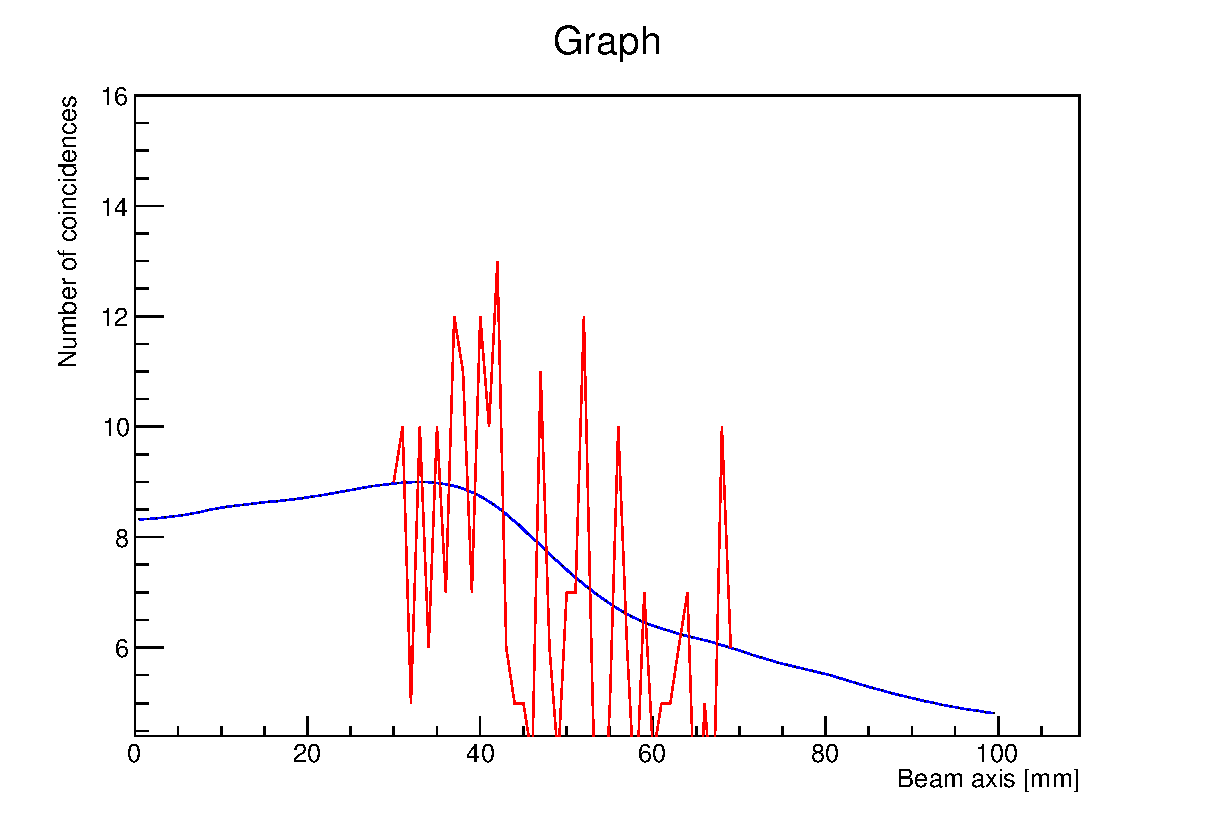
\includegraphics[width=0.33\textwidth]{./Figure/2017-08-02_Poisson_Nurbs_1e8_Article_LC.eps}}
 \subfloat[\label{fig:fig_Estimation_Camera_CC_NURBS_Poisson_LC}]{\includegraphics[width=0.33\textwidth]{./Figure/line_cone_NURBS.png}}
 %\subfloat[\label{fig:fig_Estimation_Camera_CC_NURBS_Poisson_MLEM}]{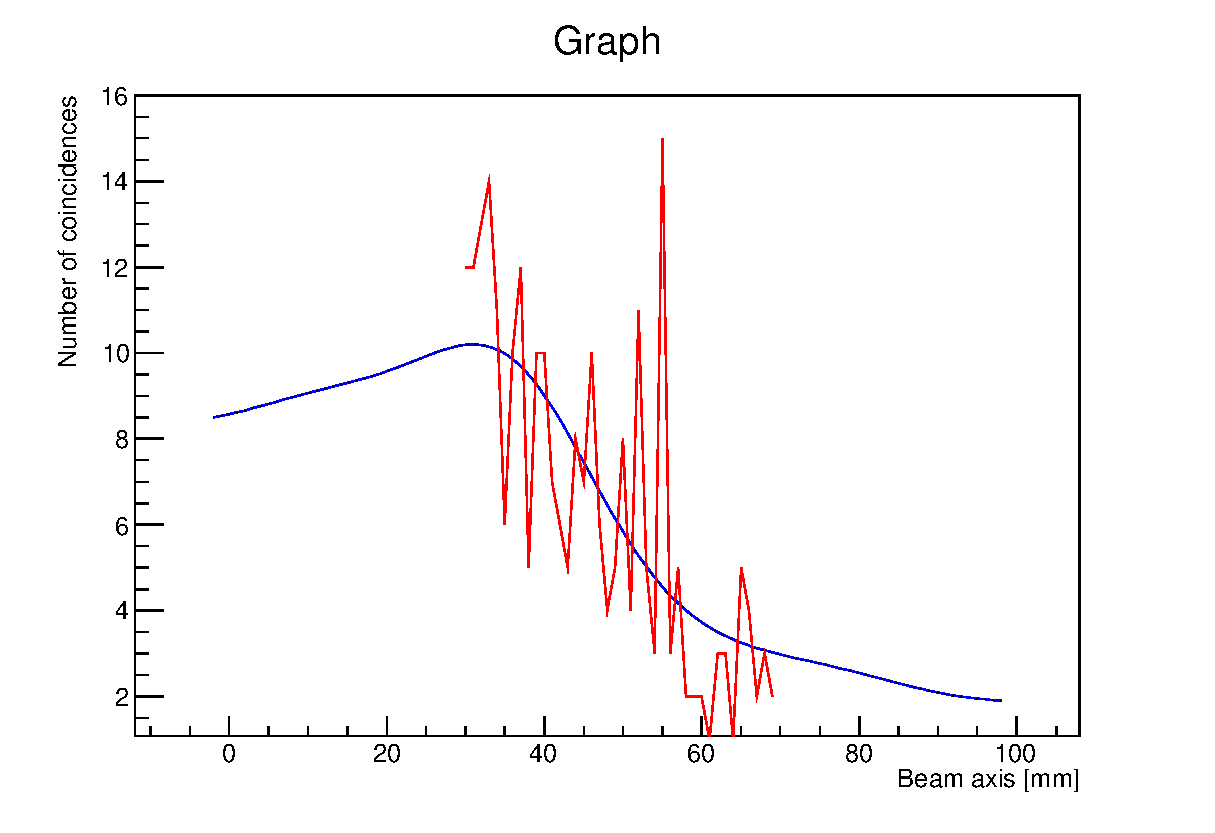
\includegraphics[width=0.33\textwidth]{./Figure/2017-08-02_Nurbs_Poisson_1e8_Article_MLEM.eps}}\\
 \subfloat[\label{fig:fig_Estimation_Camera_CC_NURBS_Poisson_MLEM}]{\includegraphics[width=0.33\textwidth]{./Figure/MLEM_NURBS.png}}\\
  %\subfloat[\label{fig:fig_Results_Chi2_Distribution_Variation_CC_simulation_Hadronth_LC}]{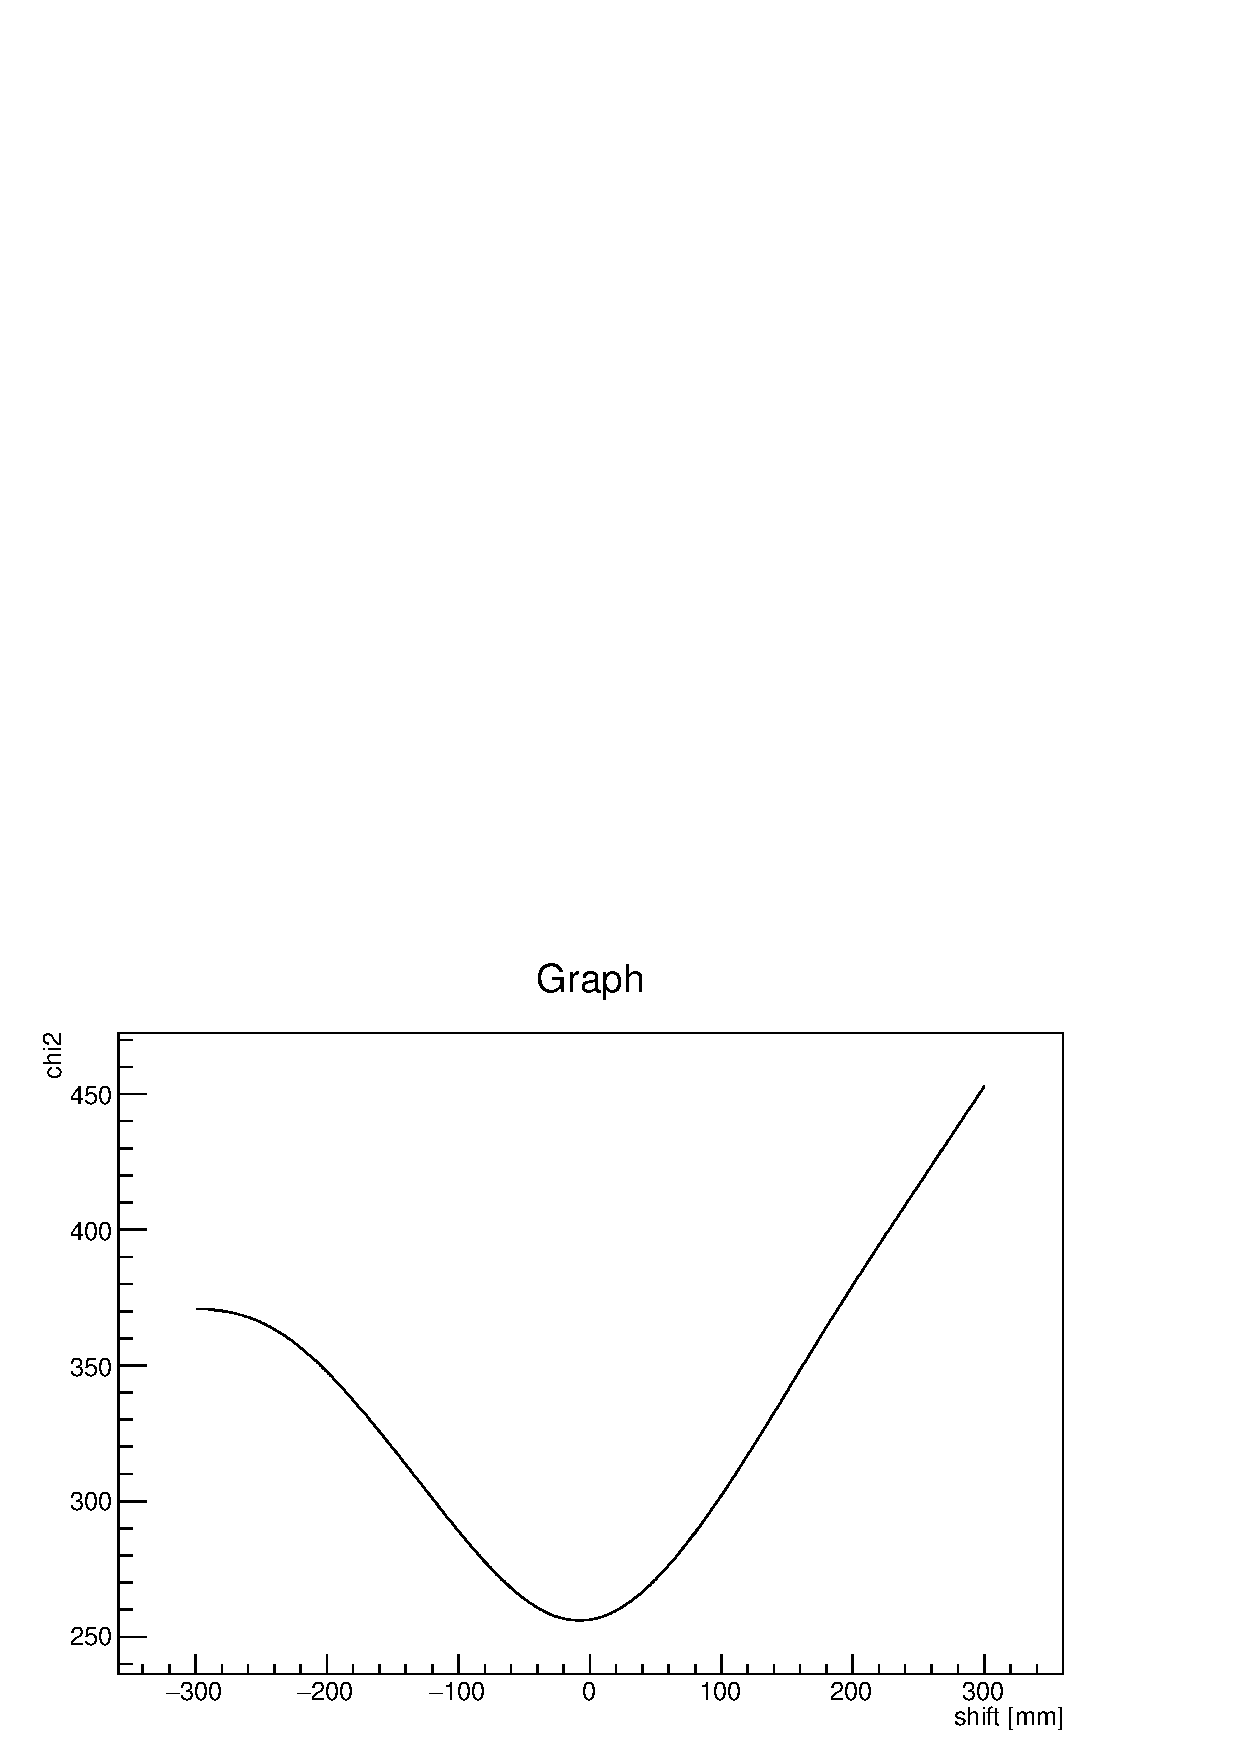
\includegraphics[width=0.33\textwidth]{./Figure/2017-08-02_Distribution_Chi2_1e8_LC.pdf}}
  \subfloat[\label{fig:fig_Results_Chi2_Distribution_Variation_CC_simulation_Hadronth_LC}]{\includegraphics[width=0.33\textwidth]{./Figure/chi2_linecone.png}}
 %\subfloat[\label{fig:fig_Results_Chi2_Distribution_Variation_CC_simulation_Hadronth_MLEM}]{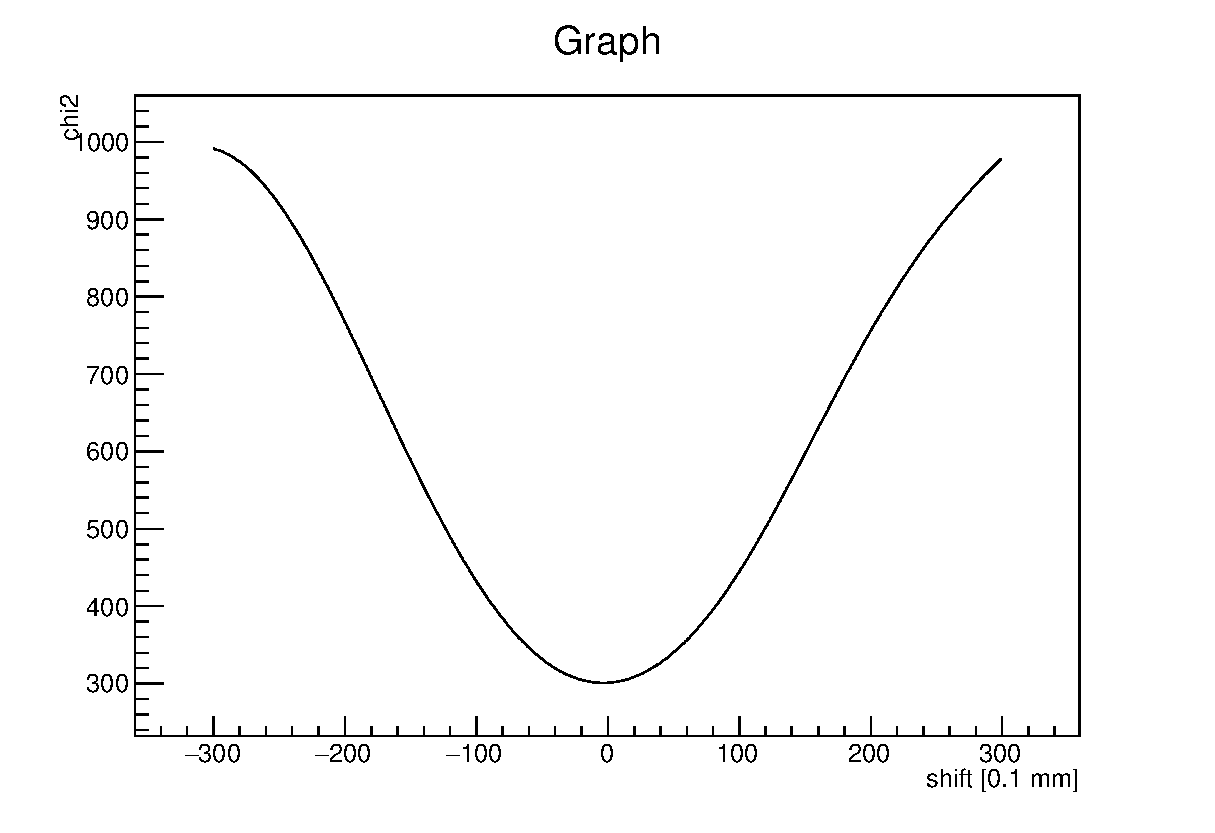
\includegraphics[width=0.33\textwidth]{./Figure/2017-08-02_Distribution_Chi2_Results_binning_1mm_ShiftNurbs0_1mm_1e8_article_MLEM.eps}}\\
 \subfloat[\label{fig:fig_Results_Chi2_Distribution_Variation_CC_simulation_Hadronth_MLEM}]{\includegraphics[width=0.33\textwidth]{./Figure/chi2_MLEM.png}}\\
  %\subfloat[\label{fig:fig_Results_Precision_Distribution_Variation_CC_simulation_Hadronth_LC} ]{\includegraphics[width=0.33\textwidth]{./Figure/2017-08-02_Distribution_finale_1e8_Article_LC.pdf}}
  \subfloat[\label{fig:fig_Results_Precision_Distribution_Variation_CC_simulation_Hadronth_LC} ]{\includegraphics[width=0.33\textwidth]{./Figure/deviation_linecone.png}}
 %\subfloat[\label{fig:fig_Results_Precision_Distribution_Variation_CC_simulation_Hadronth_MLEM} ]{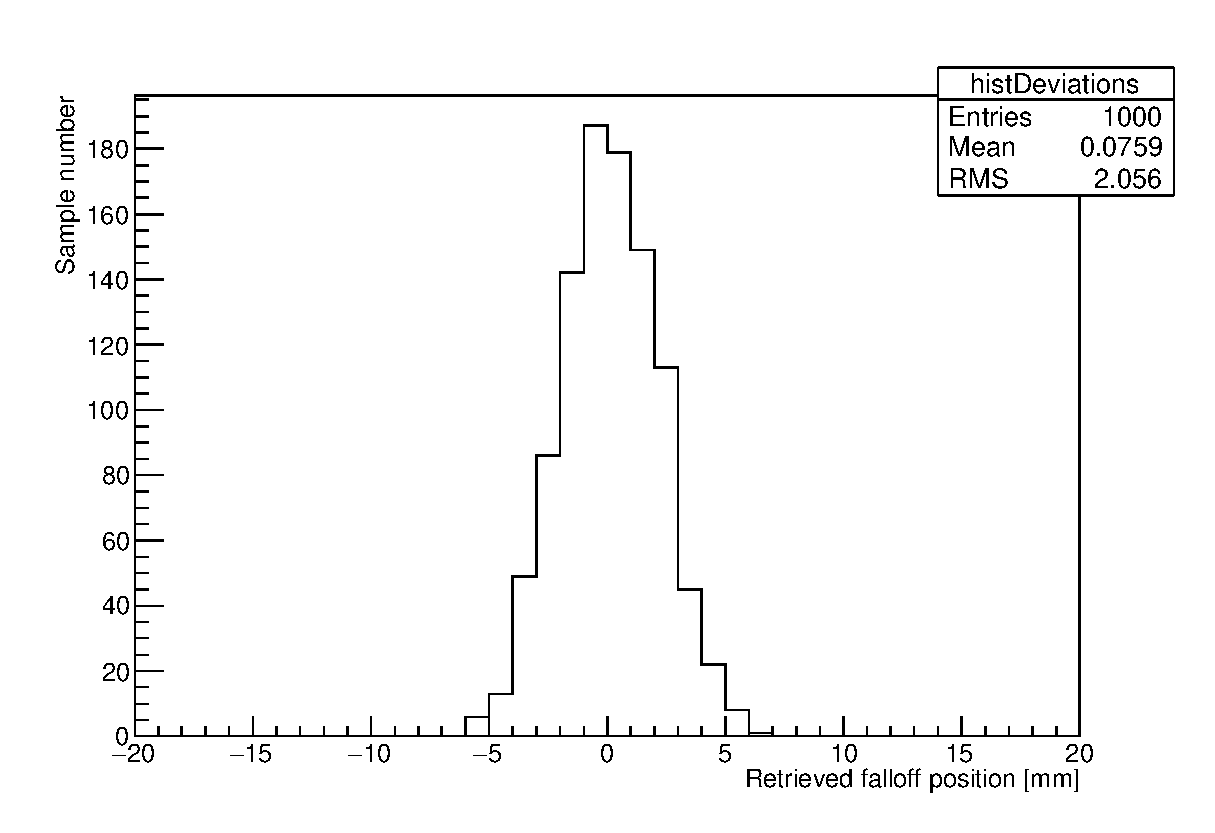
\includegraphics[width=0.33\textwidth]{./Figure/2017-08-02_FallOff_Results_binning_1mm_ShiftNurbs0_1mm_1e8_Article_MLEM.eps}}
 \subfloat[\label{fig:fig_Results_Precision_Distribution_Variation_CC_simulation_Hadronth_MLEM} ]{\includegraphics[width=0.33\textwidth]{./Figure/deviation_MLEM.png}}
\caption{Data processing comparison for the same proton simulation with the line cone algorithm (left column) and the LM-MLEM algorithm (right column). The first row gives the reconstructed profile for $10^{10}$ incident protons. The second row shows the reference curve (blue) and the curve obtained with a $10^8$ incident protons subset. The third row shows the $\chi^2$ distribution for one data subset. The last row represents the distribution of the minimal calculated shifts for 1000 subsets at the same statistics of $10^8$ incident protons.}
\end{figure}




\section{Results}

\subsection{CC efficiency}

	\begin{figure} [!hbtp]	
	\centering
	\caption{Detection efficiency function of the Compton Camera position.}	
	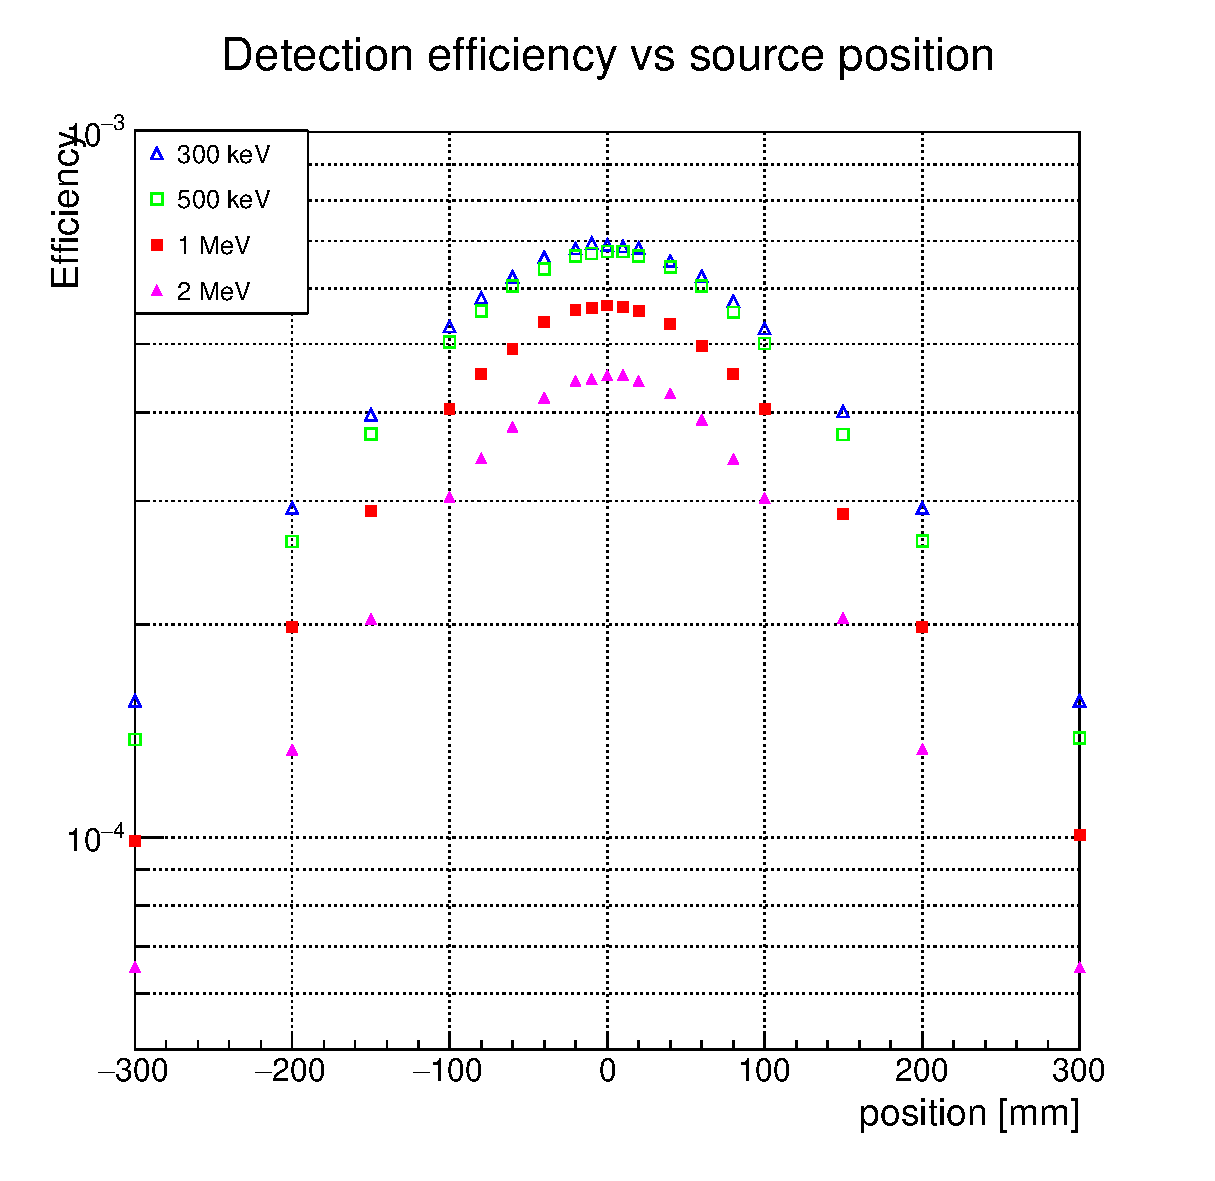
\includegraphics[width=0.7\textwidth]{./Figure/2017-06-26_Efficiency_CC_articles.eps}
	\end{figure}


\subsection{Beam intensity }
Je traite les simulations pour une statistique de $10^{8}$ pour les protons et une statistique de $2\times10^{5}$ pour les ions carbone.\newline
J'assigne à chaque particule interagissant dans le diffuseur et l'absorbeur un num\'ero de paquet auquel elle est th\'eoriquement rattach\'ee au vu de la structure en temps choisie et de l'intensit\'e du faisceau.
The modification of the beam intensity will change the number of particles included in a bunch. For instance, at the clinical intensity in protons, there is in average 217 protons in a bunch.



The beam intensity plays an important role for the Compton camera concerning its capability to distinct events in coincidence. In the simulation, the beam intensity is modeled by an average number of particles per bunch. The exact number of particles in each bunch is given by a random draw in a Poisson distribution, where the mean value is the beam intensity chosen. The range of intensities was chosen in order to cover almost all the possibilities: from a very low beam intensity to the clinical beam intensity. Therefore, for proton and carbon ion, the lowest beam intensity is set to 0.001 particles per bunch in average and for protons goes up to 217 protons per bunch when in case of carbon ion, it goes up to 70 particles per bunch. The coincidence yields are scaled per ion incidents and the beam intensity per average ions per bunch. The true coincidences represent a coincidence in the camera by the same gamma ray. The background corresponds to all the other coincidence types.


\begin{figure} [!h]
\caption{Coincidences yield for protons (a) and carbon ions (b) in function of the beam intensity. The intensity is given for a number of incident particles per bunch.  The distinction between the filled markers and the empty ones are that the time of flight discrimination is applied in the case of empty markers.}
\subfloat[]{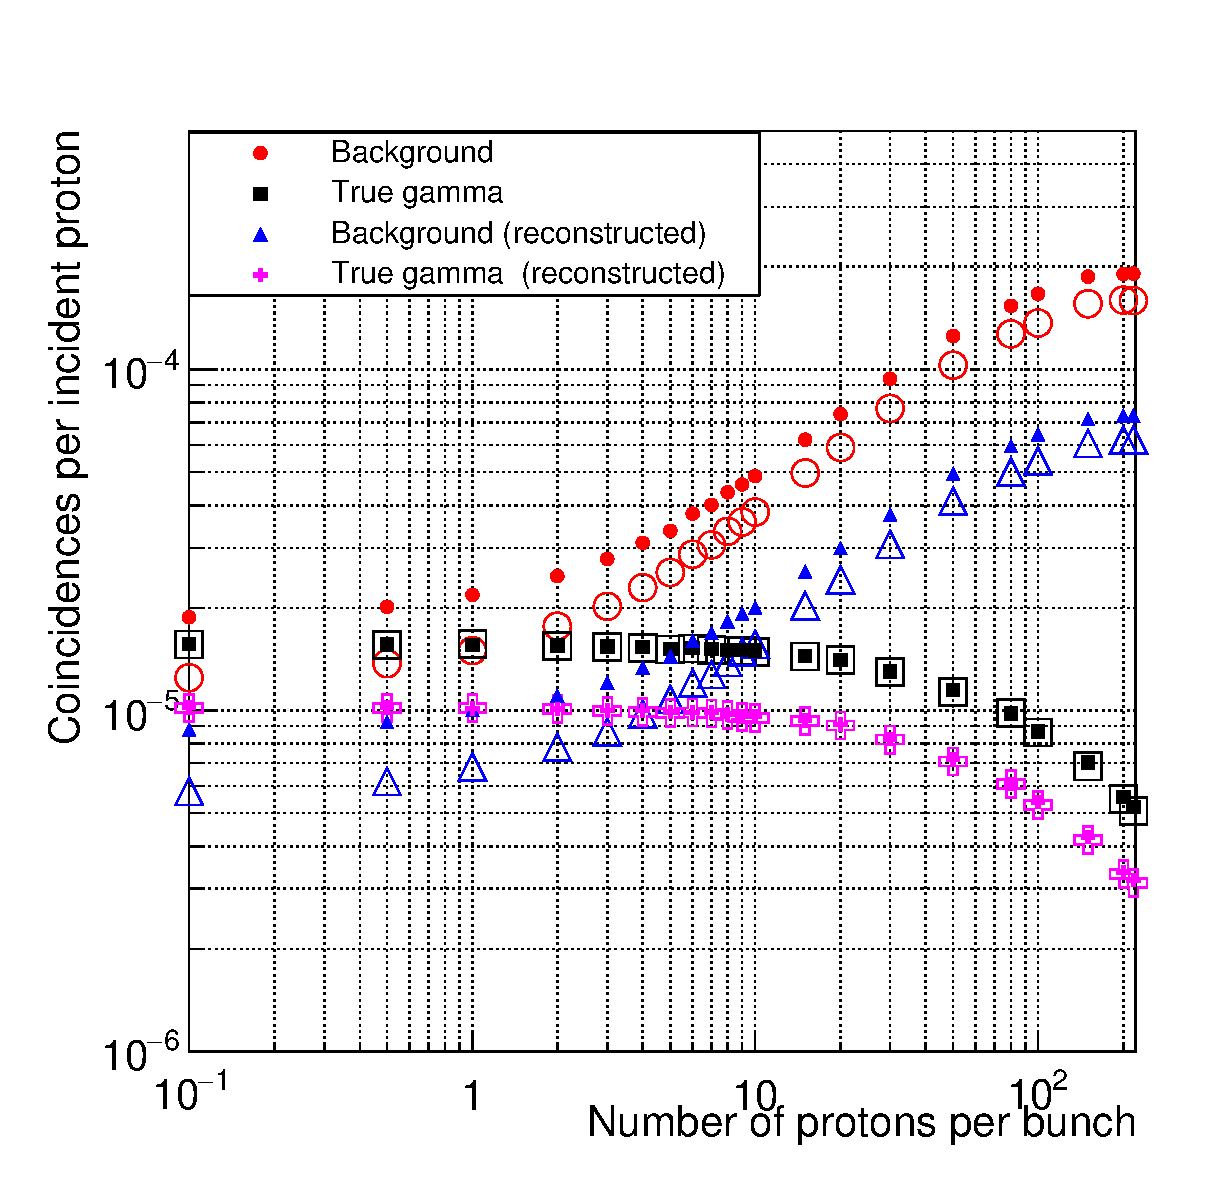
\includegraphics[width=0.5\textwidth]{./Figure/2017_06_28_Taux_coincidences_variation_protons_New_design_4EntreesLegend_LogXLogY.eps}}
 \subfloat[]{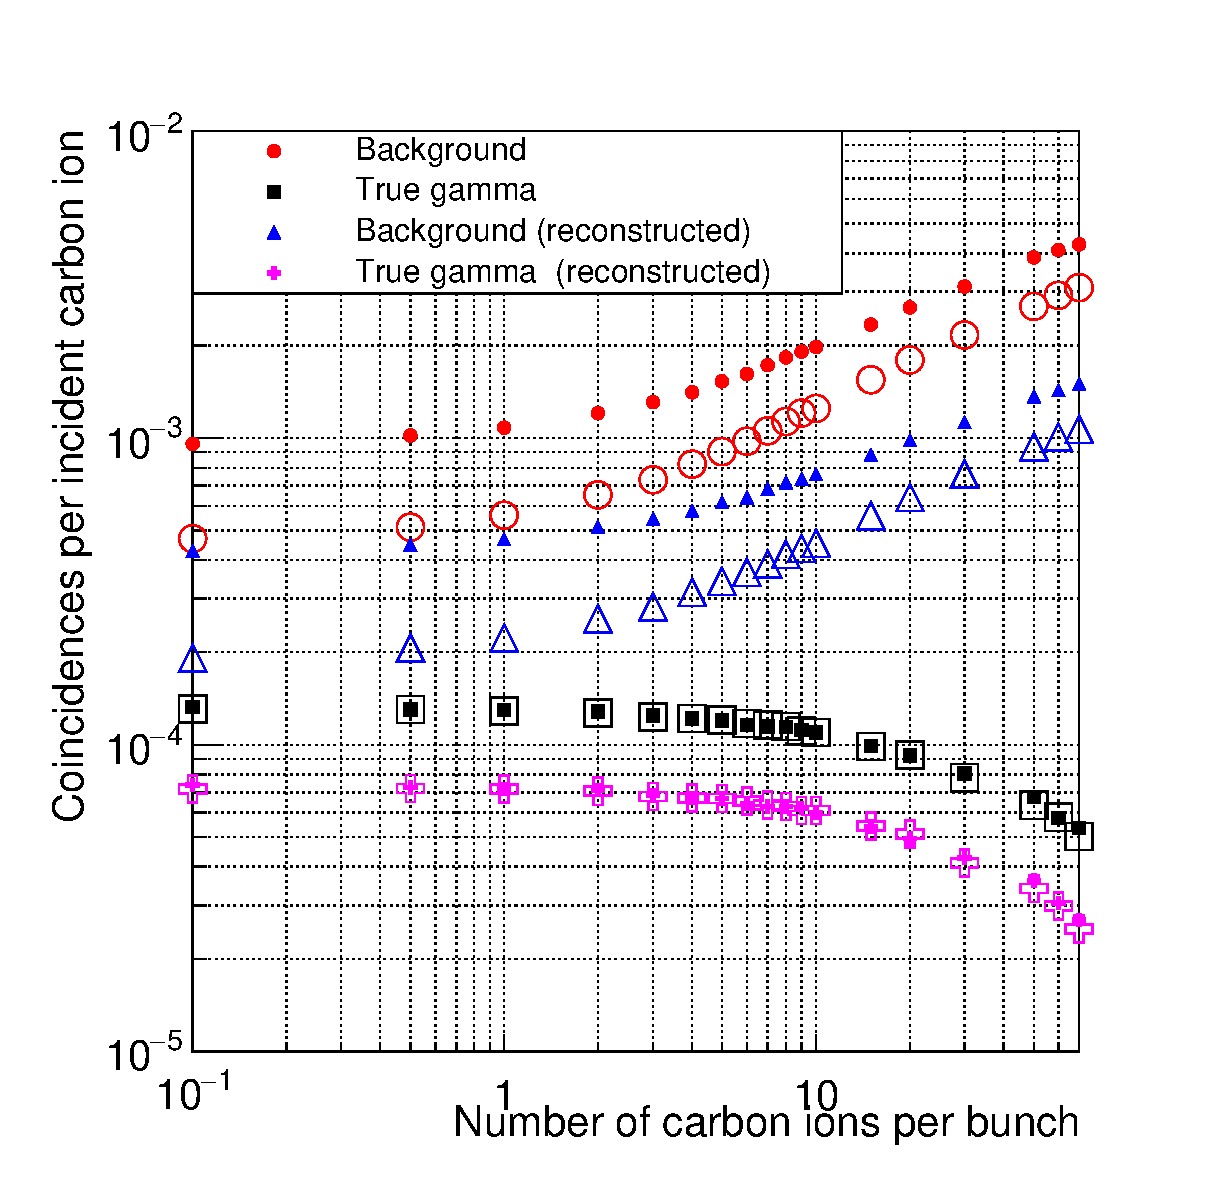
\includegraphics[width=0.5\textwidth]{./Figure/2017_06_28_Taux_coincidences_variation_carbonIons_New_design_4EntreesLegend_LogXLogY.eps}}
  \label{fig:coincidences}
\end{figure}

\newpage
At the clinical beam intensity, the high background level is mainly due to the random coincidences. In fact, the probability to detect two radiation coming from two different incident particles increases with the number of incident particles per bunch. Another issue is the single rate of events detected by each detector at those high intensities. For instance, at the clinic beam intensity in proton therapy, the single rate on the absorber is around 300 MHz and on the first silicon layer it is around 20 MHz. The current electronic front end and acquisition system are not able to treat this amount of data coming from all the detectors. As a result, it appears that it is impossible to use the Compton camera at a clinical beam intensity for the treatment monitoring in ion therapy.\newline
Nevertheless, if the intensity decreases enough to avoid almost all the random coincidences, the monitoring seems more feasible. In addition, it can be supposed that the time of flight discrimination will improve the signal to the background ratio at low intensities by suppressing the coincidences induced by charged particles. Indeed, the charged particles are slower than gamma rays which move at the light speed.\newline

\subsection{Comparaison LM-MLEM vs Line cone reconstruction}


\begin{figure} [!h]
\subfloat[]{\includegraphics[width=0.5\textwidth]{./Figure/MLEM_2D.pdf}}
 \subfloat[]{\includegraphics[width=0.5\textwidth]{./Figure/MLEM_1D.pdf}}\\
  \subfloat[]{\includegraphics[width=0.5\textwidth]{./Figure/2015_02_16_Reconstruction_coinc_160MeVProton_TOF_6ns_file0to100_zoom.pdf}}
  \label{fig:comparaison}
  \caption{Comparaison LM-MLEM vs Line cone reconstruction}

\end{figure}

%   \begin{verbatim}
% a) 2015_10_20_Volume_100x100x5_voxels_and_size_20x40x1_source_Proton160MeV_camera_50mm_stat_2175events_sans_MatriceSensibility_bordYplusmoins-3_bordXplusmoins-3_median_iteration_10.
% b) 2015_10_20_Volume_100x100x5_voxels_and_size_20x40x1_source_Proton160MeV_camera_50mm_stat_2175events_sans_MatriceSensibility_bordYplusmoins-3_bordXplusmoins-3_selectionX_20mm_Filtre_median_iteration_Profil_Y_iteration_10. 
% c)  2015_02_16_Reconstruction_coinc_160MeVProton_TOF_6ns_file0to100_zoom               
%  \end{verbatim}

\subsection{Compton camera precision}


The information given by a control device as the Compton camera has to be viable and as precise as possible. In order to estimate the precision of the Compton camera, a method is used. 

\begin{figure}[!hbtp]	
\centering
\caption{Precision function of the incident protons .}	
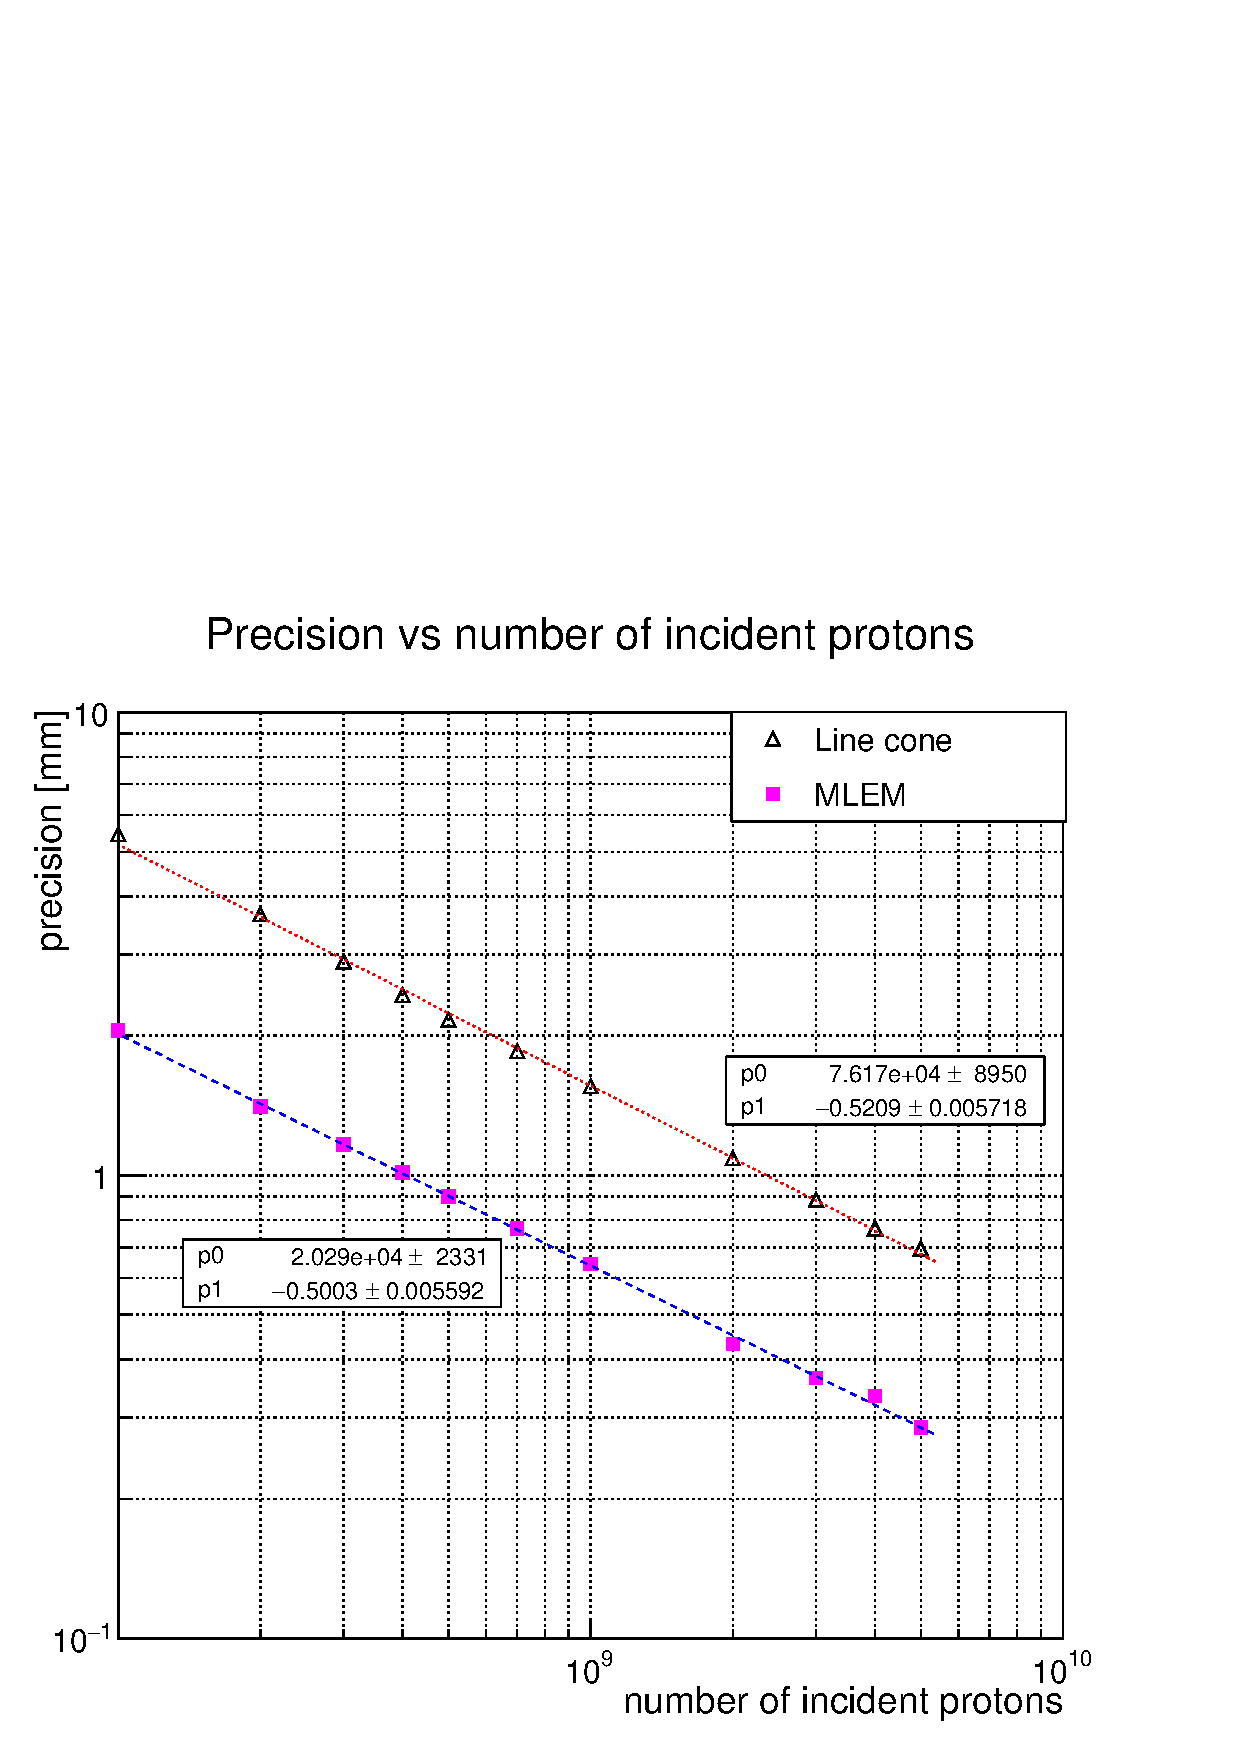
\includegraphics[width=0.7\textwidth]{./Figure/2017-08-02_Precision_Comparaison_linecone_MLEM_Article_Fit.pdf}
\end{figure}





\section{Discussion}



Therefore, the Compton camera position optimization with respect to the expected Bragg peak position appears mandatory for an efficient fall-off reconstruction.\newline

A further study showed how this effect is mainly due to the cut applied on the scatterer detector. Indeed, for low energies, below 2~MeV, the increased efficiency in the central section of the camera active surface shown in figure~\ref{fig::efficiency_study}(a) is linked to the increased relative number of photons approaching the camera with small angles. These photons are more likely undergoing Compton scattering with a reduced energy deposition, which is recorded by an ideal detector and rejected by the energy cut. The effect is all the more important as the primary gamma energy is limited, creating the peculiar energy dependence of the efficiency reduction emerged in the results in figure~\ref{fig::efficiency_study}(b).
 
Furthermore, considering the rate of single interactions per detector, the results obtained by a preliminary analysis showed, as an example, a single rate of about 300~MHz on the absorber and 20~MHz on the first scatterer planes. These rates are not compatible with the detection rate capabilities of the detector read-out chains. As a result, it appears not possible to perform a valuable treatment monitoring with the CLaRyS Compton camera at a clinical beam intensity.\newline

In the case of carbon ions, the larger amount of secondary neutron produced during the patient treatment seems to require other background rejection methods in order to lead to an advantageous signal-over-background ratio.\\

If we consider the important increase in the precision of the falloff identification given by the increased statistics, the spot grouping method seems to be promising for monitoring purpose when high accuracy is required, probably obtained in the post-treatment due to the long required reconstruction time. A sufficiently good precision is achieved on a spot basis, where the precision is about 2~mm with a MLEM reconstruction: a qualitative monitoring of each spot seems then possible. Given the long calculation time required by the MLEM algorithm, the line-cone reconstruction method, despite the reduced precision, can still be an option for on-line treatment check, when safety limit can be fixed in order to exclude severe deviation from the treatment planning and an interruption of the dose delivery in real time can be foreseen.          



% 
% \section*{Acknowledgments}
% 
% This work is supported by the FP7-ENVISION program WP3, the FP7-ENTERVISION program, the FP7- ULICE program, the ANR Gamhadron project, the Rhone-Alpes Regional Program for Hadrontherapy Research, the MI2B GDR and the LabEx PRIMES.

\section*{References}
\bibliographystyle{apalike}
\bibliography{Biblio_13.bib}



\end{document}

